%%%%%%%%%%%%%%%%%%%% author.tex %%%%%%%%%%%%%%%%%%%%%%%%%%%%%%%%%%%
%
% sample root file for your "contribution" to a contributed volume
%
% Use this file as a template for your own input.
%
%%%%%%%%%%%%%%%% Springer %%%%%%%%%%%%%%%%%%%%%%%%%%%%%%%%%%


% RECOMMENDED %%%%%%%%%%%%%%%%%%%%%%%%%%%%%%%%%%%%%%%%%%%%%%%%%%%
\documentclass[graybox]{svmult}

% choose options for [] as required from the list
% in the Reference Guide

\usepackage{mathptmx}       % selects Times Roman as basic font
\usepackage{helvet}         % selects Helvetica as sans-serif font
\usepackage{courier}        % selects Courier as typewriter font
\usepackage{type1cm}        % activate if the above 3 fonts are
                            % not available on your system
\usepackage{makeidx}         % allows index generation
\usepackage{graphicx}        % standard LaTeX graphics tool
                             % when including figure files
\usepackage{multicol}        % used for the two-column index
\usepackage[bottom]{footmisc}% places footnotes at page bottom
\usepackage{amsmath,amssymb,latexsym}

%% change footnote numbers to symbols
\renewcommand{\thefootnote}{\fnsymbol{footnote}}
\newcommand{\bxi}{\ensuremath{\boldsymbol{\xi}}}
\newcommand{\btheta}{\ensuremath{\boldsymbol{\theta}}}
% see the list of further useful packages
% in the Reference Guide

\makeindex             % used for the subject index
                       % please use the style svind.ist with
                       % your makeindex program

%%%%%%%%%%%%%%%%%%%%%%%%%%%%%%%%%%%%%%%%%%%%%%%%%%%%%%%%%%%%%%%%%%%%%%%%%%%%%%%%%%%%%%%%%

\begin{document}

\title*{Inference for Coupled SDE: Metropolis Algorithms via Density Tracking by Quadrature}
\titlerunning{Inference for Coupled SDE: Metropolis and DTQ Algorithms}
% Use \titlerunning{Short Title} for an abbreviated version of
% your contribution title if the original one is too long
\author{Harish S. Bhat, R. W. M. A. Madushani, and Shagun Rawat}

% Use \authorrunning{Short Title} for an abbreviated version of
% your contribution title if the original one is too long
\institute{Harish S. Bhat \at University of California Merced, 5200 N. Lake Rd., Merced, CA, USA \\ \email{hbhat@ucmerced.edu}
\and R. W. M. A. Madushani \at University of California Merced, 5200 N. Lake Rd., Merced, CA, USA \\ \email{rmadushani@ucmerced.edu}
\and Shagun Rawat \at University of California Merced, 5200 N. Lake Rd., Merced, CA, USA \\ \email{srawat2@ucmerced.edu}
}

%
% Use the package "url.sty" to avoid
% problems with special characters
% used in your e-mail or web address
%
\maketitle

\abstract*{We develop a Metropolis algorithm to perform Bayesian inference for models given by coupled stochastic differential equations. A key challenge in developing practical algorithms is the computation of the likelihood. We address this problem through the use of a fast method to track the probability density function of the stochastic differential equation.  The method applies quadrature to the Chapman-Kolmogorov equation associated with a temporal discretization of the stochastic differential equation.  The inference method can be adapted to scenarios in which we have multiple observations at one time, multiple time series, or observations with large and/or irregular temporal spacing.  Computational tests show that the resulting Metropolis algorithm is capable of efficient inference for an electrical oscillator model.}

\section{Introduction}
\label{sec:1}
Stochastic Differential Equations (SDE) are a widely used powerful mathematical tool to model real-world phenomena. However, parameter inference of SDE models is still a 
very challenging problem, due to the fact that the likelihood function is generally unknown for the case where time-discrete observations are available \cite{sorensen2004parametric, iacus2009simulation, fuchs2013inference}. Most existing parametric inference methods for discretely observed SDE require inter-observation time to be small, to track the transition density for the discrete time observations. As a way to facilitate approximation of the transition density for parametric inference for large inter-observation times, Bayesian methods are used to simulate missing values of the observations to form a high-frequency data set. In situations where the likelihood function is either analytically unavailable or computationally prohibitive to evaluate, Bayesian inference of SDE makes use of likelihood-free methods such as Approximate Bayesian Computation \cite{Picchini2014}, variational methods \cite{Archambeau2007a, Vrettas2015}, and/or Gaussian processes \cite{Archambeau2007, Ruttor2013}.

%SDE have application in areas epidemiology, mechanics, genetics, population biology, systems biology, molecular dynamics, geostatistics,social sciences, economics and finance. (include why parameter estimation is important, existing methods and the challenge of computation of the likelihood)

In our work we have developed a Markov Chain Monte Carlo Method (MCMC) algorithm for Bayesian inference of parameters in SDE.  The MCMC algorithm is derived using a Metropolis scheme; our innovation is to evaluate the log likelihood efficiently using density tracking by quadrature (DTQ).  The DTQ method applies quadrature to the Chapman-Kolmogorov equation associated with a time-discretization of the original SDE \cite{BhatMadu2016}. For the case of scalar SDE, the DTQ method's density function converges to the true density of the SDE at a rate that is linear in the time step.  The method we have developed is applicable to the case where inter-observation times are large and/or irregular.  In this paper, we present a Metropolis algorithm for Bayesian inference of unknown parameters of a 2-D SDE.

\section{Derivation of the Numerical Method}
\label{sec:2}
% Always give a unique label
% and use \ref{<label>} for cross-references
% and \cite{<label>} for bibliographic references
% use \sectionmark{}
% to alter or adjust the section heading in the running head
Let $W_{1,t}$ and $W_{2,t}$ denote two independent Wiener processes with $W_{1,0} = W_{2,0} = 0$ almost surely. In this work, we deal with coupled SDE of the form:
\begin{subequations}
\label{eqn:sde}
\begin{align}
\mathrm{d}X_{1,t} &= f_1(\mathbf{X}_t, \btheta)\mathrm{d}t + g_1(\mathbf{X}_t, \btheta) \mathrm{d}W_{1,t} \\
\mathrm{d}X_{2,t} &= f_2(\mathbf{X}_t, \btheta)\mathrm{d}t + g_2(\mathbf{X}_t, \btheta) \mathrm{d}W_{2,t}.
\end{align}
\end{subequations}
Here $\mathbf{X}_t = (X_{1,t}, X_{2,t})$ is a two-dimensional stochastic process. For $j=1, 2$, we refer to $f_j$ and $g_j$ as, respectively, drift and diffusion functions.  Both drift and diffusion functions may depend on a parameter vector $\boldsymbol{\theta}\in \mathbb{R}^{N}$.

Our goal is to infer the parameter vector $\btheta$ from direct observations of $\mathbf{X}_t$.  Suppose that at a sequence of times $0 = t_0 < t_1 < \cdots < t_M = T$, we have observations $\mathbf{x} := \{({x}_{1,m},{x}_{2,m})\}_{m=0}^M$.  Here $\mathbf{x}_m = ({x}_{1,m},{x}_{2,m})$ is a sample of $\mathbf{X}_{t_m}$.  In this paper, we will assume equispaced temporal observations, i.e., $t_m = m \Delta t$ for fixed step size $\Delta t > 0$.  We make this assumption purely for notational simplicity; the method we describe can be easily adapted for nonequispaced temporal observations.  We refer to $\Delta t$ as the time step of the data.

The posterior density of the parameter vector given the observations is
$p(\btheta \, | \, \mathbf{x})  \propto p( \mathbf{x} \, | \, \btheta)  p(\btheta)$,
where $p( \mathbf{x} \, | \, \btheta)$ is the likelihood and $p(\btheta)$ is the prior.  We discretize the SDE (\ref{eqn:sde}) in time using the Euler-Maruyama scheme:
\begin{subequations}
\label{eqn:discretesde}
\begin{align}
X_1^{n+1} &= X_1^{n} + f_1(X_1^n, X_2^n, \btheta)h + g_1(X_1^n, X_2^n,  \btheta) \sqrt{h} Z_1^{n} \\
X_2^{n+1} &= X_2^{n} + f_2(X_1^n, X_2^n,\btheta)h + g_2(X_1^n, X_2^n,\btheta) \sqrt{h} Z_2^{n}.
\end{align}
\end{subequations}
Here $h > 0$ is a fixed time step, the time step of our numerical method.  We shall choose $h$ to be a fraction of $\Delta t$, i.e., $F h = \Delta t$ for integer $F \geq 2$.  The random variables $X_i^n$ for $i=1,2$ are approximations of $X_{i,n h}$.  The $Z_i^n$ are independent and identically distributed random variables, normally distributed with mean $0$ and variance $1$, i.e., $Z_i^n \sim \mathcal{N}(0,1)$.

Let $\widetilde{p}(\mathbf{x} \, | \, \btheta)$ denote the likelihood under the discrete-time model (\ref{eqn:discretesde}), an approximation to the true likelihood $p(\mathbf{x} \, | \, \btheta)$.  Note that (\ref{eqn:discretesde}) describes a discrete-time Markov chain.  By the Markov property, the likelihood $\widetilde{p}(\mathbf{x} \, | \, \btheta)$ factors and we can write:
\begin{equation}
\label{eqn:markovfactor}
p(\mathbf{x} \, | \, \btheta) \approx \widetilde{p}(\mathbf{x} \, | \, \btheta) = \prod_{m=0}^{M-1} \widetilde{p}(\mathbf{x}_{m+1} \, | \, \mathbf{x}_m, \btheta).
\end{equation}
The term $\widetilde{p}(\mathbf{x}_{m+1} \, | \, \mathbf{x}_m, \btheta)$ is the transition density for (\ref{eqn:discretesde}), from state $\mathbf{x}_m$ at time $t_m$ to state $\mathbf{x}_{m+1}$ at time $t_{m+1}$.  This suggests a numerical method for computing this density, which we explore in the next subsection.
 
\subsection{Density Tracking by Quadrature (DTQ)}
\label{subsec:2-1}
Equation (\ref{eqn:discretesde}) describes a Markov chain over a continuous state space.  If we let $\widetilde{p}^n(x_1,x_2 \, | \, \btheta)$ denote the joint probability density function of $X_1^n$ and $X_2^n$ given $\btheta$, then the Chapman-Kolmogorov equation associated with (\ref{eqn:discretesde})  is
\begin{equation}
\label{eqn:chapman}
\widetilde{p}^{n+1}(x_1,x_2 \, | \, \btheta) = \int_{y_1,y_2 \in \mathbb{R}^2} K(x_1,x_2,y_1,y_2; \btheta) \widetilde{p}^n(y_1,y_2 \, | \, \btheta) \, dy,
\end{equation}
where
\begin{align}
&K(x_1,x_2,y_1,y_2; \theta) = \widetilde{p}^{{n+1} | {n}}(x_1,x_2 | y_1,y_2,\theta) \nonumber\\
&= (2 \pi \sigma_1^2)^{-1/2} \exp \left[ -(x_1 - \mu_1)^2/(2 \sigma_1^2) \right] (2 \pi \sigma_2^2)^{-1/2} \exp \left[ -(x_2 - \mu_2)^2/(2 \sigma_2^2) \right]\nonumber.
\end{align}
Here $\mu_1 = y_1 + f_1(y_1,y_2; \theta) h,  \mu_2 = y_2 + f_2(y_1,y_2; \theta) h,  \sigma_1^2 = g_1^2(y_1,y_2; \theta) h$ and  $\sigma_2^2 = g_2^2(y_1,y_2; \theta) h$. That is, $K(x_1,x_2,y_1,y_2; \theta)$ is the conditional density of $X_1^{n+1}$ and $X_2^{n+1}$ given $X_1^n = y_1$, $X_2^n = y_2$ and $\btheta = \theta$, evaluated at the point $(x_1,x_2)$.  The fact that the conditional density is a product of normal distributions with means $\mu_1, \mu_2$ and variances $\sigma_1^2, \sigma_2^2$ can be shown using (\ref{eqn:discretesde}) together with the fact that $X_1^{n+1}$ and $X_2^{n+1}$ are conditionally independent given $X_1^n$ and $X_2^n$. This conditional independence is a direct consequence of having two independent random variables $Z_1^n$ and $Z_2^n$ in (\ref{eqn:discretesde}).

The crux of the DTQ method is to apply quadrature to (\ref{eqn:chapman}) to evolve an initial density forward in time.  Consider a spatial grid with fixed spacing $k > 0$ and grid points $x_1^i = ik$, $x_2^j = jk$, $y_1^{i'} = i'k$, and $y_2^{j'} = j'k$.  Then we apply the trapezoidal rule in both the $y_1$ and $y_2$ variables to obtain:
\begin{equation}
\hat{p}^{n+1}(x_1^i, x_2^j ;\theta) = k^2 \sum\limits_{i' = -\infty}^{\infty} \sum\limits_{j' = -\infty}^{\infty} K(x_1^i, x_2^j, y_i^{i'}, y_2^{j'}; \theta) ) \hat{p}^n(y_1^{i'}, y_2^{j'}; \theta)
\end{equation}
It is unnecessary to sum over all of $\mathbb{Z}^2$.  We know that a two-dimensional Gaussian decays to zero far from its mean.  Since the mean $(\mu_1,\mu_2)$ is approximately $(y_1,y_2)$, we sum only from $y_1 = x_1 - \gamma k$ to $y_1 = x_1 + \gamma k$ and similarly for $y_2$:
\begin{equation}
\label{eqn:phatalg}
\hat{p}^{n+1}(x_1^i, x_2^j;\theta ) = k^2 \sum\limits_{i' = i - \gamma}^{i+ \gamma} \sum\limits_{j' = j-\gamma}^{j+\gamma} K(x_1^i, x_2^j, y_i^{i'}, y_2^{j'}; \theta) \hat{p}^n(y_1^{i'}, y_2^{j'}; \theta)
\end{equation}
We now have our method to evaluate $\widetilde{p}(\mathbf{x}_{m+1} \, | \, \mathbf{x}_m, \btheta)$.  Let us take $n=0$ in (\ref{eqn:phatalg}) to correspond to the time $t_m$.  We start with the deterministic initial condition $\mathbf{X}^0 = \mathbf{x}_m$, corresponding to the density $\widetilde{p}^0(\mathbf{x}) = \delta(\mathbf{x} - \mathbf{x}_m)$.  Inserting this point mass into (\ref{eqn:chapman}), we obtain a Gaussian density for $\widetilde{p}^1(\mathbf{x})$.  For each $i,j \in [-y_M/k, y_M/k]$, we set
$$
\hat{p}^1(x_1^i, x_2^j; \theta) = \widetilde{p}^1(x_1^i, x_2^j; \theta).
$$
Now that we have $\hat{p}^1$, we use (\ref{eqn:phatalg}) repeatedly to compute $\hat{p}^2$, $\hat{p}^3$, and so on until we reach $\hat{p}^F$.  The object $\hat{p}^F$ is then a spatially discrete approximation of the transition density from time $t_m$ to time $t_m + Fh = t_{m+1}$.  Interpolating this density at the point $\mathbf{x}_{m+1}$, we compute a numerical approximation of $\widetilde{p}(\mathbf{x}_{m+1} \, | \, \mathbf{x}_m, \btheta)$, as required for the likelihood function.

\subsection{Metropolis Algorithm}
\label{subsec:2-2}
Once we have an efficient method to compute the likelihood, we can use the method in a Metropolis algorithm to sample from the posterior. In the Metropolis algorithm, we construct an auxiliary  Markov chain $\lbrace \hat{\vec{\btheta}}_N\rbrace_{N\geq 0}$ which is designed to have an invariant distribution given by the posterior $p(\btheta \, | \, \mathbf{x})$. This Markov chain is constructed as $\hat{\vec{\btheta}}_{N+1} = \hat{\vec{\btheta}}_N + Z_{N+1}$,
where $Z_{N+1}$ is a random vector with dimension equal to that of the parameter vector $\btheta$.  In this paper, we choose all components of $Z_{N+1}$ to be independent normal random variables with known means and variances.

The Metropolis algorithm is as follows:
\begin{itemize}
\item Choose value $q_0$ for $\hat{\vec{\btheta}}_{0}$.
\item Once the values $q_0, \cdots, q_N$ of $\hat{\vec{\btheta}}_{0},\cdots,\hat{\vec{\btheta}}_{N}$ have been found:
\begin{itemize}
\item Generate a proposal value $q_{N+1}^{*}$ from the auxiliary Markov chain:
$q_{N+1}^{*} = q_{N} + Z_{N+1}$.
\item Calculate the ratio $\rho = \frac{p(q_{N+1}^{*}  \, | \, \mathbf{x})}{p(q_N \, | \, \mathbf{x})}$, where $p(q_{N+1}^{*}  \, | \, \mathbf{x}) \approx \widetilde{p}(\mathbf{x} \, | \, q_{N+1}^{*}) p(q_{N+1}^{*}) = p(q_{N+1}^{*}) \prod_{m=0}^{M-1} \widetilde{p}(\mathbf{x}_{m+1} \, | \, \mathbf{x}_m, q_{N+1}^{*})$. Now each term $\widetilde{p}(\mathbf{x}_{m+1} \, | \, \mathbf{x}_m, q_{N+1}^{*})$ can be computed using the DTQ method
discussed in Section \ref{subsec:2-1}.
\item Sample a uniform random variable $u_N \sim \mathcal{U}(0,1)$.  If $\rho > u_N$ set $\hat{\vec{\btheta}}_{N+1} = q_{N+1}^{*}$; in this case, the proposal is accepted. Else set $\hat{\vec{\btheta}}_{N+1} = q_{N}$ and the proposal is rejected.
\end{itemize}
\end{itemize}
Once we have obtained all the samples $q_0, q_1, \cdots, q_N$ from the Metropolis algorithm, we discard a sufficient number of initial samples to ensure the Markov chain has converged to its invariant distribution.

\section{Numerical Results}
\label{sec:3}
We implement the Metropolis algorithm in R. Inside the Metropolis algorithm, we evaluate the  likelihood function using the DTQ method, which is implemented in C++ as an R package. To test the performance of our method, we consider the SDE
\begin{equation}
\label{eqn:sdeapplication}
\mathrm{d}X_{1,t} =  -\frac{X_{2,t}}{L}\mathrm{d}t + \frac{s_1^2}{L} \mathrm{d}W_{1,t}, \qquad
\mathrm{d}X_{2,t} = \frac{X_{1,t}}{C}\mathrm{d}t + \frac{s_2^2}{C} \mathrm{d}W_{2,t}.
\end{equation}
This system describes a noisy electrical oscillator with one inductor (with inductance $L$) and one capacitor (with capacitance $C$).  The dependent variables $X_{1,t}$ and $X_{2,t}$ represent, respectively, the current and voltage of the circuit at time $t$.

Our goal here is to test the performance of the algorithm using simulated data.  To generate this data, we start with known values of the parameters $L$, $C$, $s_1$, and $s_2$.  Using a fixed initial condition $(X_{1,0},X_{2,0})$, we then use the Euler-Maruyama method to step (\ref{eqn:sdeapplication}) forward in time until a final time $T > 0$.  When we carry out this time-stepping, we use a step size of $0.001$ and then retain only those samples at times $t_m = m \Delta t$, from $m = 0$ to $m = M$, where $M \Delta t = T$.

For the tests presented here, the known values of the parameters are $L = C = (2 \pi)^{-1}$ and $s_1 =  s_2 = .4/\sqrt{2 \pi}$.  The simulated data is taken over two periods of the oscillator ($T = 2$) with a full resolution of $\Delta t = 0.01$.  By, for example, taking every other row of this data set, we can obtain data with a resolution of $\Delta t = 0.02$.

Using the samples $\{ \mathbf{x}_m \}_{m=0}^M$ thus constructed, we run the Metropolis algorithm. 
Because capacitance and inductance are physically constrained to be positive, we take $1/L = \theta_1^2$, $1/C = \theta_2^2$, $s_1^2/L = \theta_3^2$, and $s_2^2/C = \theta_4^2$.  In this way, each $\theta_j$ is allowed to take a random walk on $\mathbb{R}$ rather than be restricted to the positive half of the real line.  For each $\theta_j$, we use a diffuse Gaussian prior with mean $0$ and standard deviation $100$.  For the proposal distribution $Z_{N+1}$ in the auxiliary Markov chain, we choose i.i.d. Gaussians with mean $0$ and standard deviation $0.35$.

For the tests presented here, we infer only one parameter, $\theta_1$, keeping the other parameters fixed at their known values.  When we run the Metropolis algorithm, we discard the first $100$ samples and retain the next $1000$ samples.  For each value of $\Delta t$ and the DTQ time step $h$, we compute both the mean of the samples of $\theta_1^2$ and the mode of the kernel density estimate of $\theta_1^2$.  We compare these values against the true value of the parameter $1/L = 2 \pi$ and record the relative errors as, respectively, $e_1$ and $e_2$ in the following table:
\begin{center}
\begin{tabular}{llll}
$\Delta t$ & $h$ & $e_1$ (relative error of mean) & $e_2$ (relative error of mode) \\ \hline
$0.04$ & $0.04$ & $6.1\%$ & $7.6\%$ \\
$0.04$ & $0.02$ & $0.54\%$ & $6.8\%$ \\
$0.04$ & $0.01$ & $5.1\%$ & $1.1\%$ \\
$0.02$ & $0.02$ & $12\%$ & $14\%$ \\
$0.02$ & $0.01$ & $4.9\%$ & $2.3\%$
\end{tabular}
\end{center}
When $h = \Delta t$, only one step of the method described in Section \ref{subsec:2-1} is required to go from time $t_m$ to $t_{m+1}$.  This step does not use any quadrature at all---one merely evaluates (\ref{eqn:chapman}) using a point mass for the density at time $t_m$.  The resulting likelihood function is a product of Gaussians.  On the other hand, when $h$ is strictly less than $\Delta t$, we must use quadrature (i.e., the actual DTQ method) to step forward in time from $t_m$ to $t_{m+1}$.

To visualize the results, we present the following plot of the posterior densities of $1/L$ corresponding to the first three lines of the table above.  The true value of $1/L = 2 \pi$ is indicated by the dashed black line.  The posterior mode for $h = 0.01$ is indicated by the solid black line:
\vspace{-0.6in}
\begin{center}
\includegraphics[width=3in,angle=270]{densities.eps}
\end{center}
\vspace{-0.1in}
Overall, the findings above support our view that using the DTQ method to compute the likelihood yields more accurate posteriors than using a purely Gaussian likelihood.

\begin{acknowledgement}
We gratefully acknowledge support from UC Merced's Committee on Research.
\end{acknowledgement}

\bibliographystyle{spmpsci}
\bibliography{HMS2016}

\end{document}

%$$
%p^{n+1}(\mathbf{x};\theta) = \int_{y_1=x_1-\Gamma}^{y_1=x_1+\Gamma} \int_{y_2=x_2-\Gamma}^{y_2=x_2+\Gamma} K(x_1,x_2,y_1,y_2; \theta) p^n(\mathbf{x};\theta).
%$$

% To infer the unknown parameters $L, C, \sigma_1,$ and $\sigma_2$ in (\ref{eqn:sdeapplication}) we use simulated data of $X_{1,t}$, and $X_{1,t}$ as our observations. To simulate observations we use Euler-Maryama  sampling method after fixing the unknown parameters to some known values. For $1 \leq m \leq M$, let us approximate $t_m$ by $t_m \approx (n_m) h$ where $n_m = \lfloor t_m / h \rfloor$, an integer.  We make this approximation because, while we do want to allow the data to be taken at irregular times---perhaps with large gaps---we want to apply the Euler-Maruyama approximation on a fine, equispaced grid.


